\section{Создание механизма 
сглаживания и фильтрации данных акселерометра и 
гироскопа (Агаев Фархат)}

Моей главной задачей являлось написть фильтр, 
который сможет сгладить данные и избавиться от шума.
Чтобы применить правильный фильтр нужно понять природу шума, 
почему датчик акселерометра искажает данные.
\begin{figure}[H]
    \begin{center}
        \begin{tabular}{cc}
            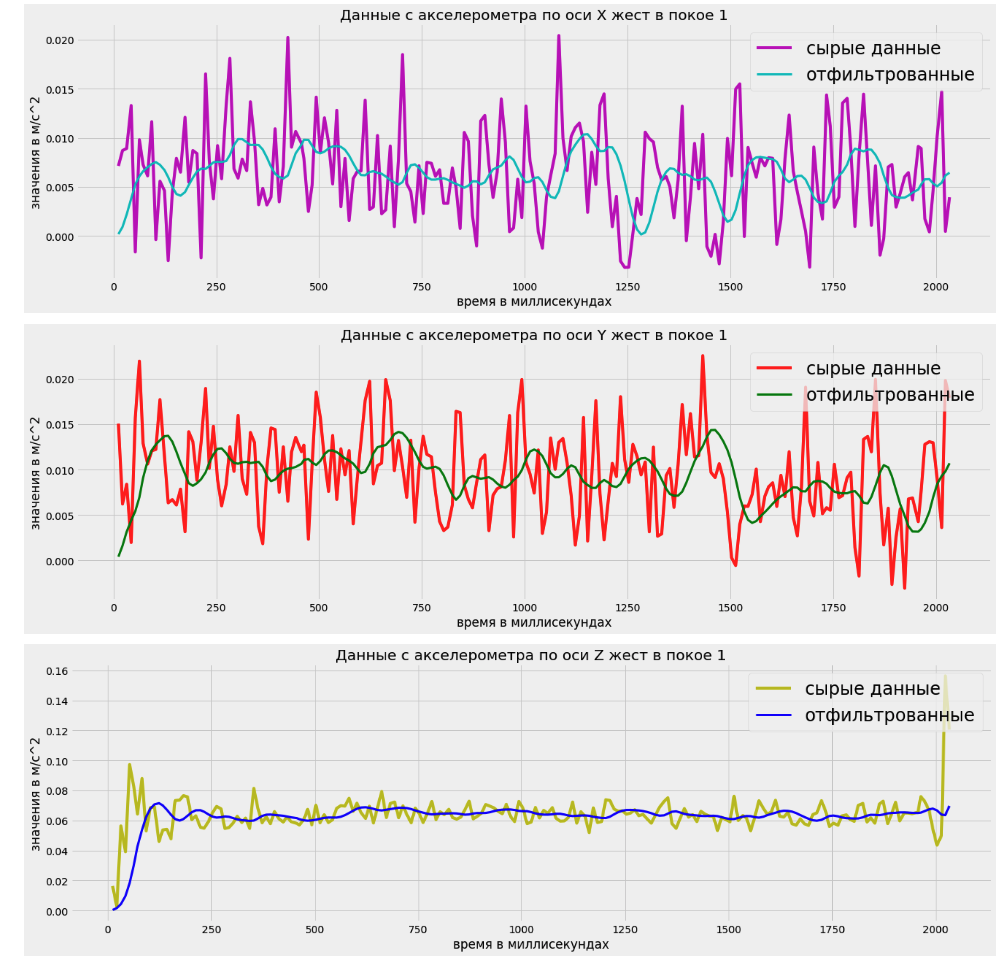
\includegraphics[width=1\textwidth]{farim/relax} & 
        \end{tabular}
    \end{center}
\end{figure}

\subsection{Природа шума}
Для начала нарисуем график по трем осям, 
когда телефон лежит на столе, посмотрим есть какие-либо перепады

\begin{figure}[H]
    \begin{center}
        \begin{tabular}{cc}
            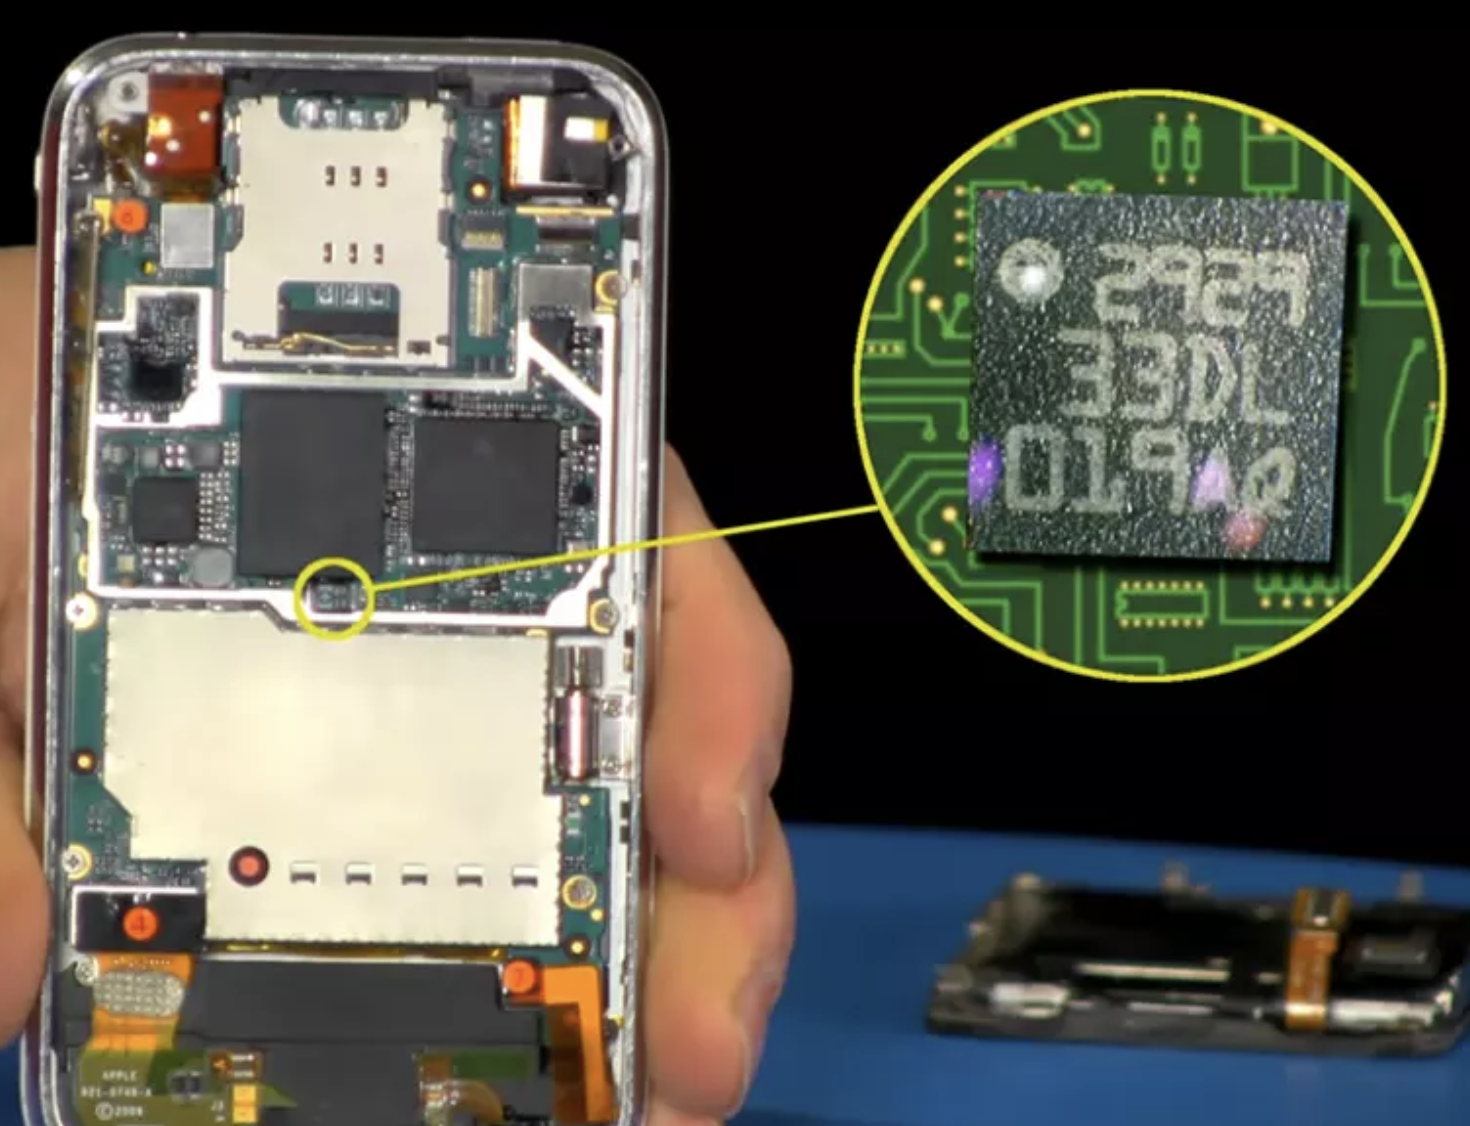
\includegraphics[width=1\textwidth]{farim/im2} & 
        \end{tabular}
    \end{center}
\end{figure}
Можно препдположить что, 
ток течет по проводам и при этом, он создаёт вокруг себя магнитное поле 
(чтобы избежать данный эффект, нужна хорошая изоляция),
которое в свою очередь и портит наши данные.
Но в телефоне датчик акселерометра - маленькая деталь, поэтому 
невозожно сделать необходимую изоляцию данного прибора (в телефон просто не поместиться).
Плюс ко всему акселерометр в 
силу своего устройства - 
достаточно неточный прибор и выдает большую погрешность.
\newpage
Теперь взглянум на график данных одного из жестов (круг)
Также посмотрим на другие жесты 
\begin{figure}[H]
    \begin{center}
        \begin{tabular}{cc}
            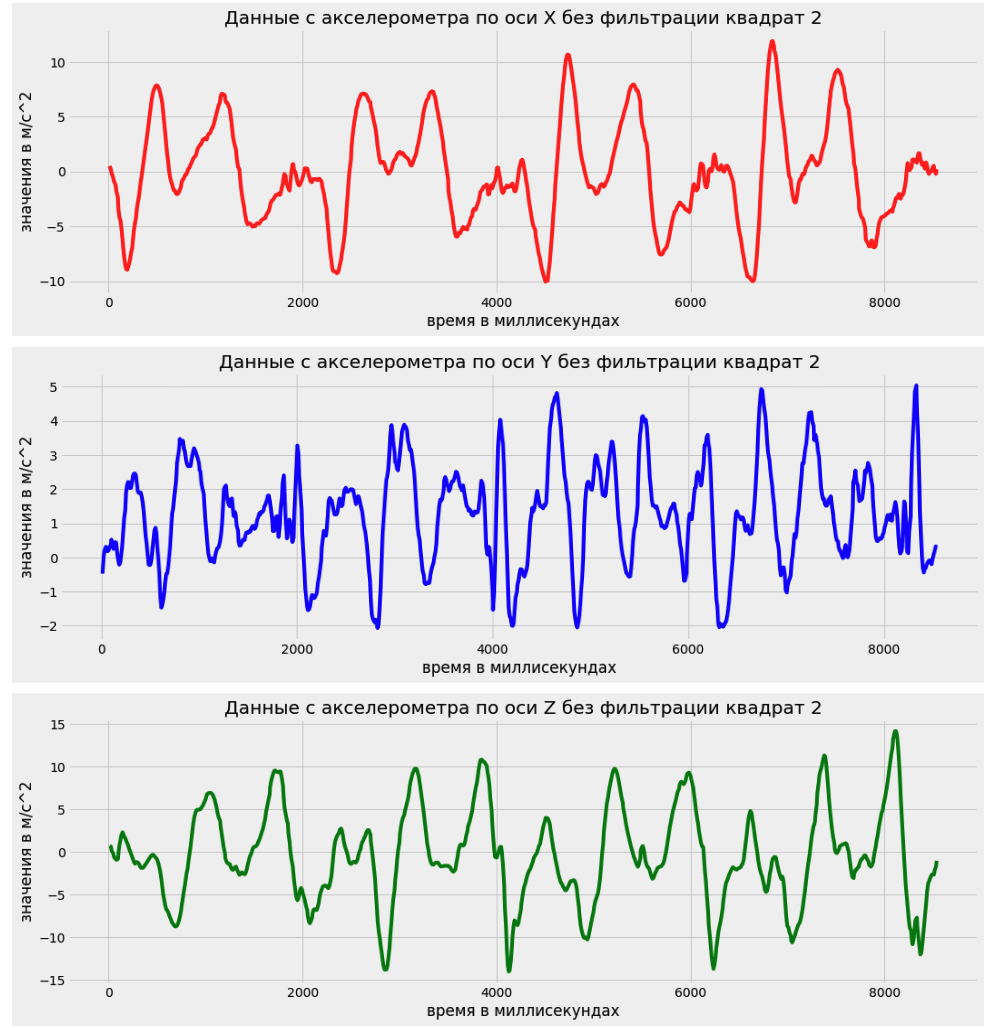
\includegraphics[width=1\textwidth]{farim/sq} & 
        \end{tabular}
    \end{center}
\end{figure}


\begin{figure}[H]
    \begin{center}
        \begin{tabular}{cc}
            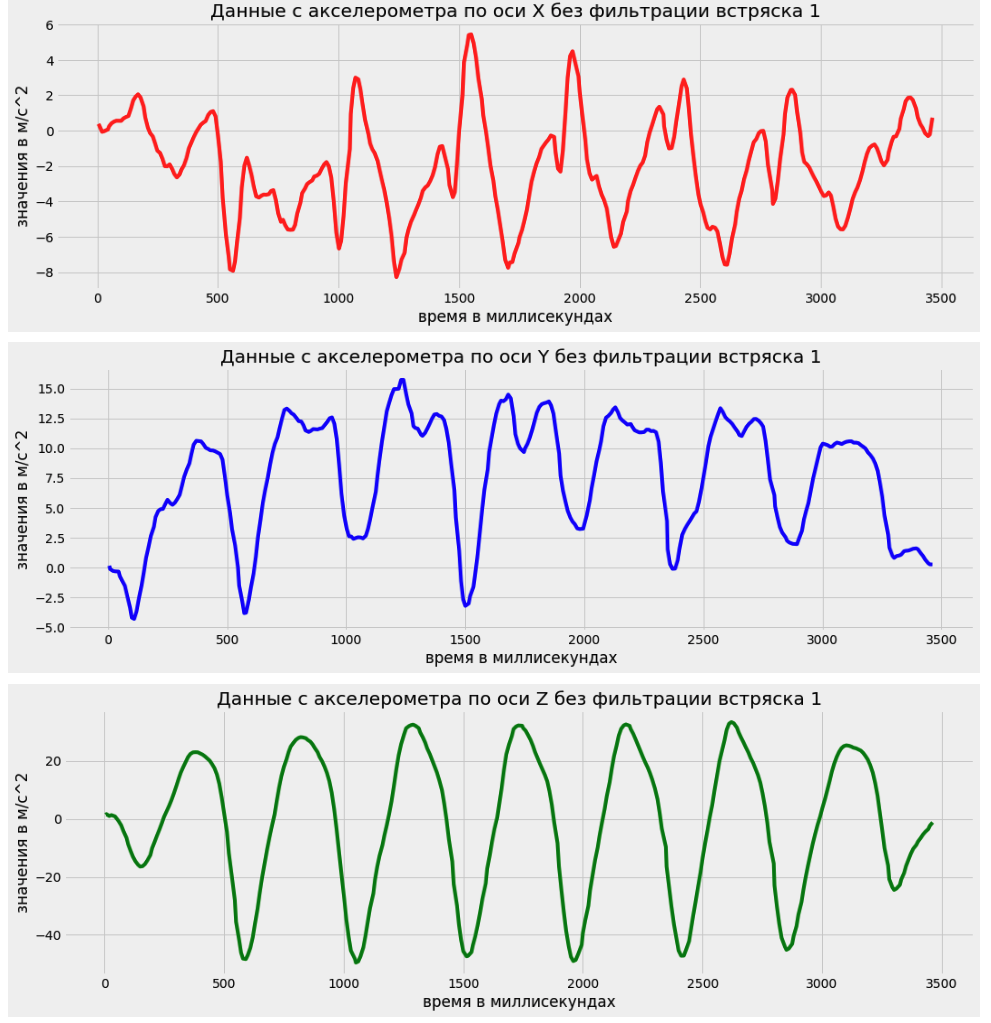
\includegraphics[width=1\textwidth]{farim/shakeeee.png} & 
        \end{tabular}
    \end{center}
\end{figure}
Исходя из графиков, мы можем понять, 
что в нашем случае идеально подойдет фильтр нижних частот, 
он сможет сгадить данные и избавиться от шума
\begin{figure}[H]
    \begin{center}
        \begin{tabular}{cc}
            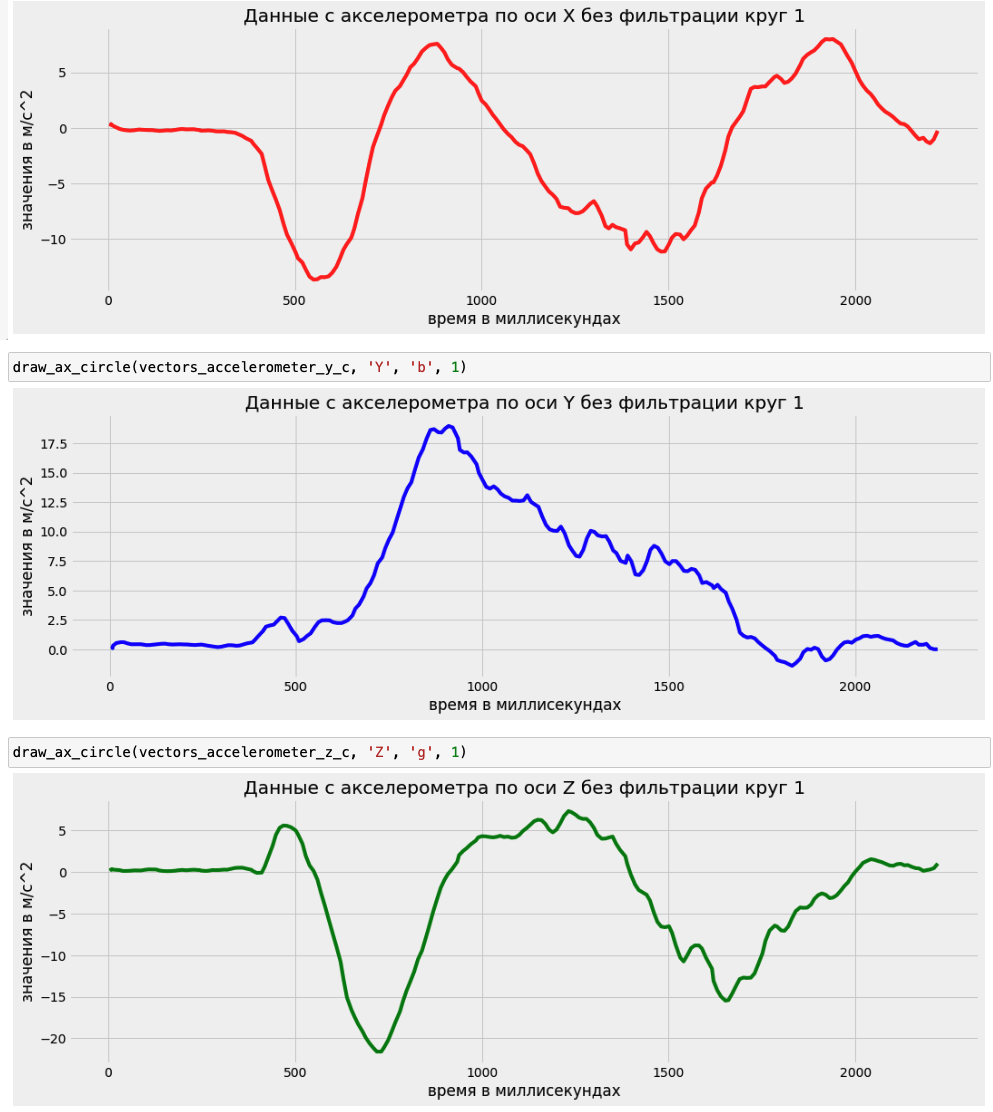
\includegraphics[width=1\textwidth]{farim/cirx} & 
        \end{tabular}
    \end{center}
\end{figure}

\newpage
\subsection{Принцип работы}

Это фильтр, который пропускает сигналы с 
частотой ниже выбранной частоты среза и 
ослабляет сигналы с частотами выше, чем частота
среза. 
Воспользуемся фильтром и посмотрим результат работы
\begin{figure}[H]
    \begin{center}
        \begin{tabular}{cc}
            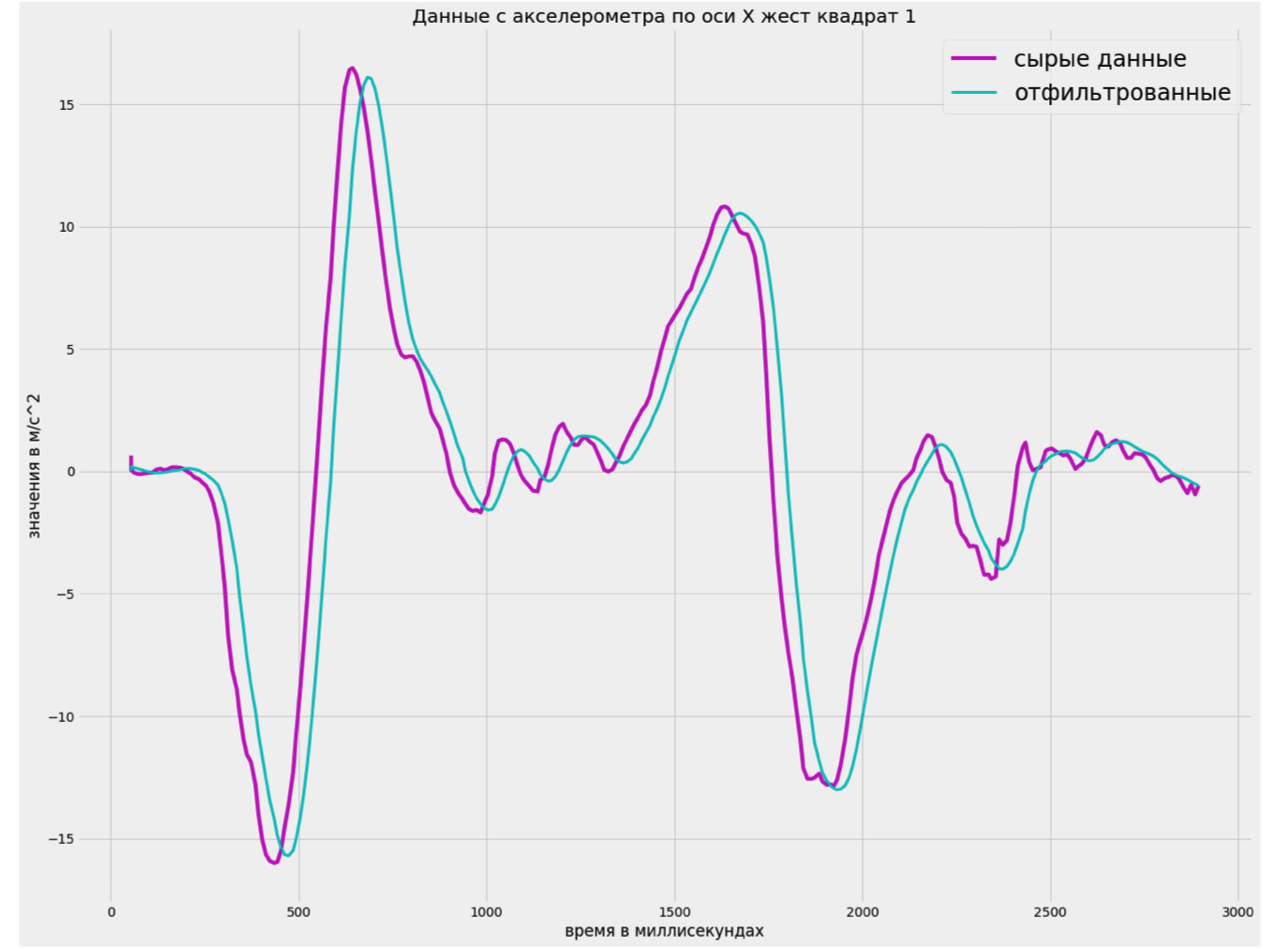
\includegraphics[width=0.7\textwidth]{farim/squares} & 
        \end{tabular}
    \end{center}
\end{figure}
\begin{figure}[H]
    \begin{center}
        \begin{tabular}{cc}
            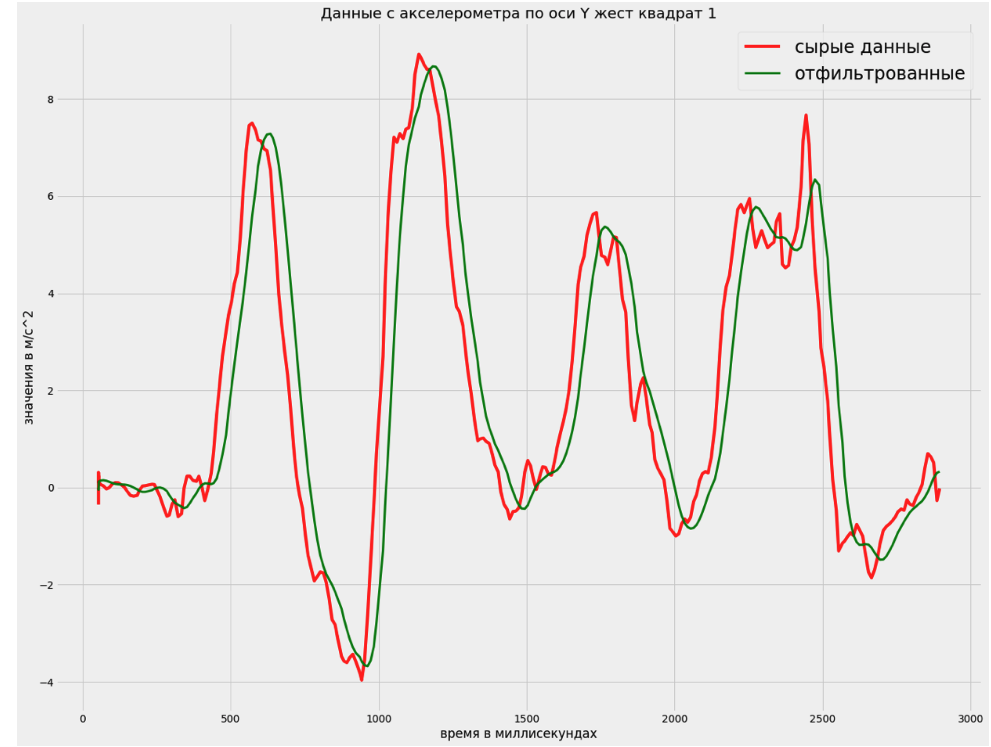
\includegraphics[width=0.7\textwidth]{farim/sqxres} & 
        \end{tabular}
    \end{center}
\end{figure}

\begin{figure}[H]
    \begin{center}
        \begin{tabular}{cc}
            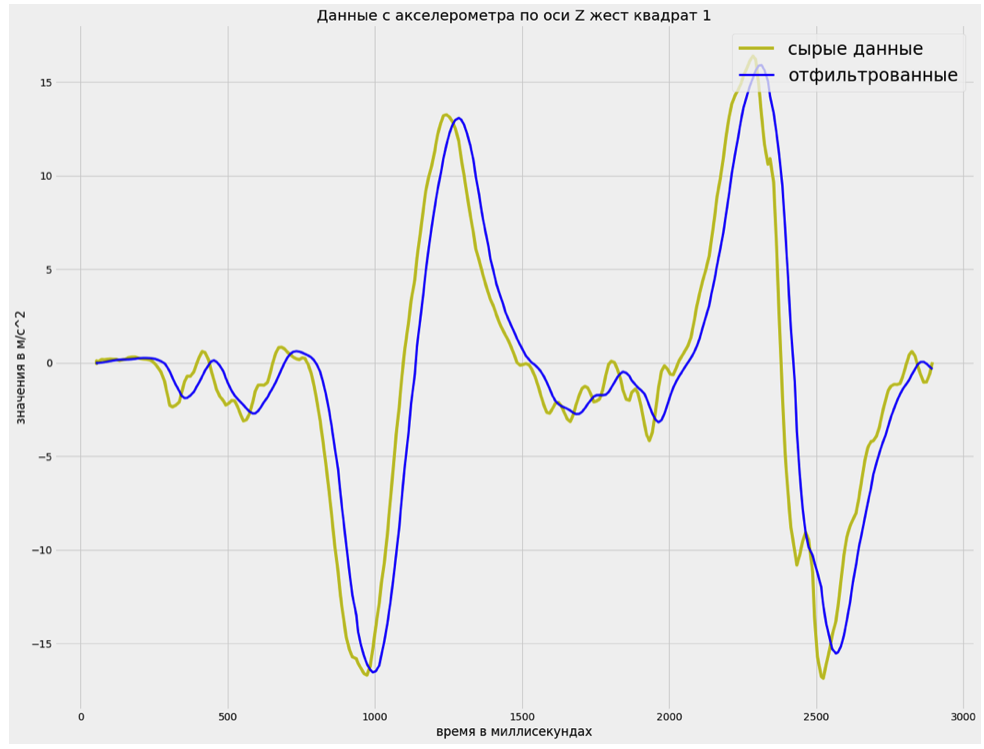
\includegraphics[width=0.75\textwidth]{farim/sqzres} & 
        \end{tabular}
    \end{center}
\end{figure}

\begin{figure}[H]
    \begin{center}
        \begin{tabular}{cc}
            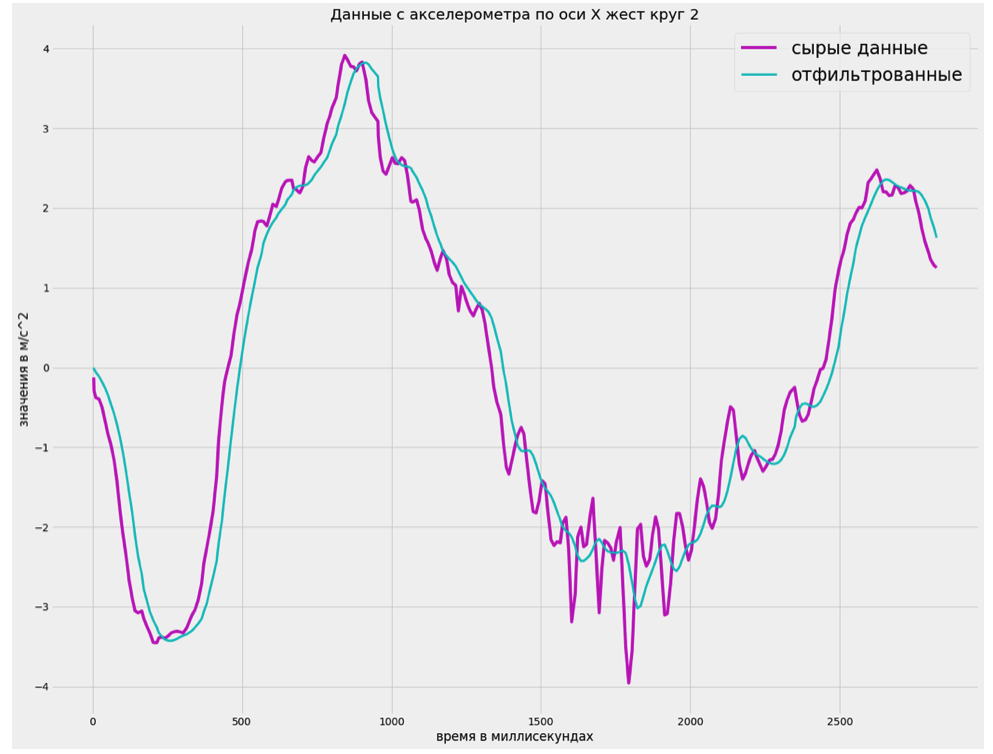
\includegraphics[width=0.75\textwidth]{farim/cirxres.png} & 
        \end{tabular}
    \end{center}
\end{figure}

\begin{figure}[H]
    \begin{center}
        \begin{tabular}{cc}
            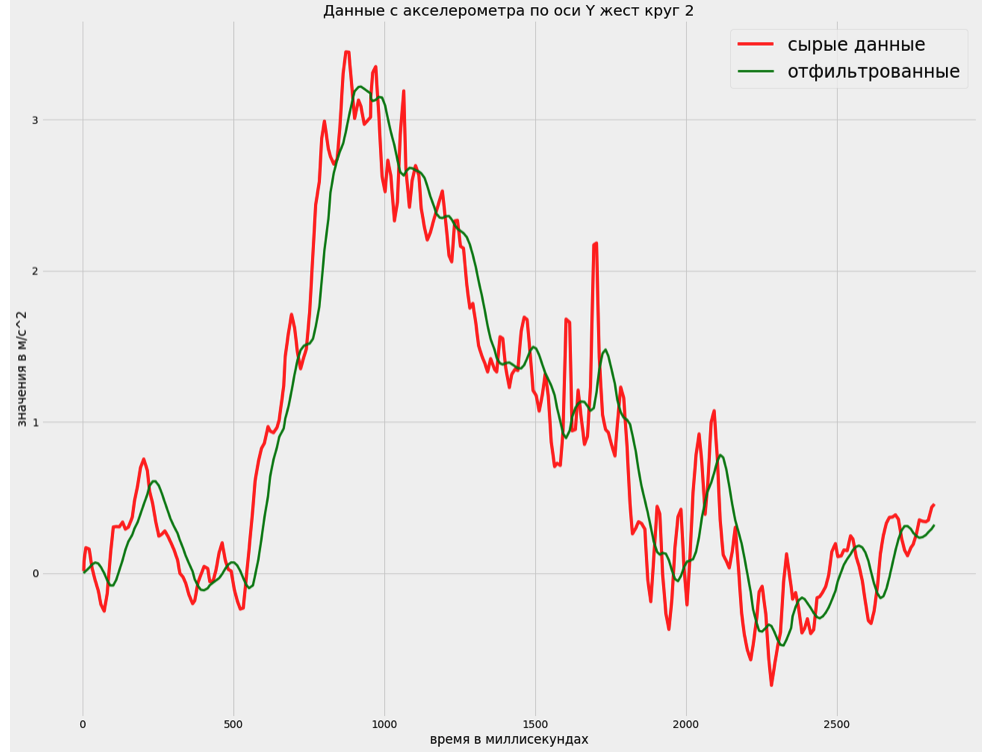
\includegraphics[width=0.75\textwidth]{farim/ciryres.png} & 
        \end{tabular}
    \end{center}
\end{figure}


\begin{figure}[H]
    \begin{center}
        \begin{tabular}{cc}
            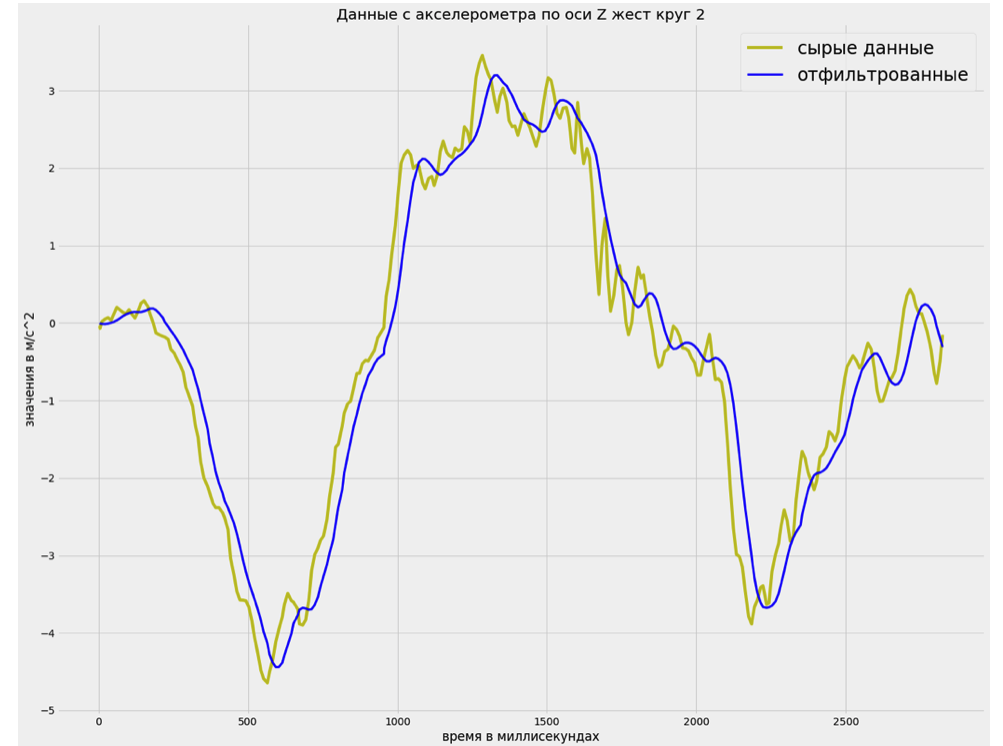
\includegraphics[width=0.75\textwidth]{farim/cirzres.png} & 
        \end{tabular}
    \end{center}
\end{figure}

\begin{figure}[H]
    \begin{center}
        \begin{tabular}{cc}
            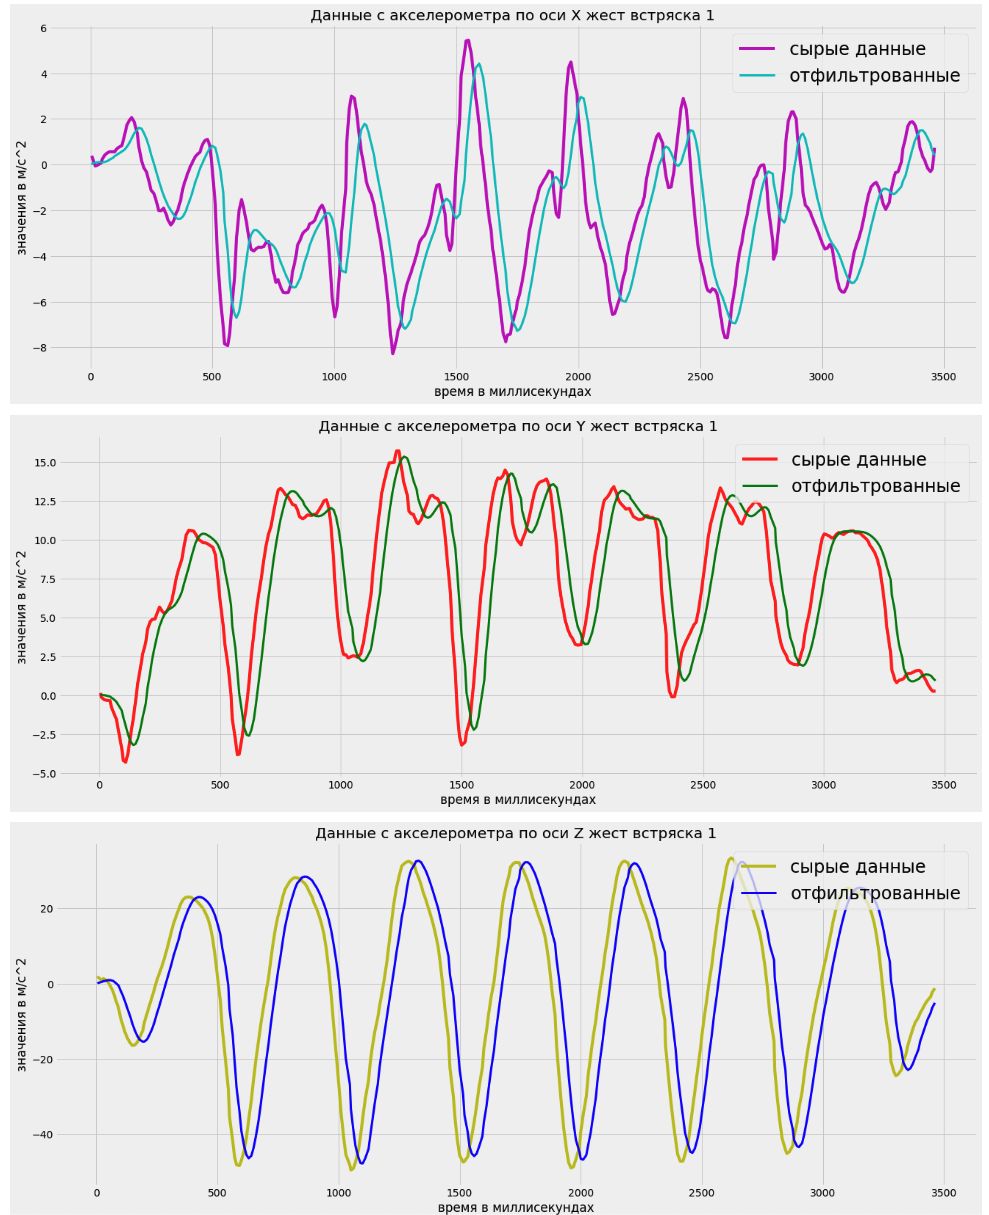
\includegraphics[width=1\textwidth]{farim/shak.png} & 
        \end{tabular}
    \end{center}
\end{figure}